% !TeX spellcheck = en_GB
\documentclass[runningheads,a4paper]{llncs}
\usepackage[utf8]{inputenc}
\usepackage[T1]{fontenc}
\usepackage{csquotes}
\usepackage[english]{babel}
\usepackage[backend=bibtex,natbib,hyperref=true,maxnames=2,style=authoryear-comp]{biblatex}
%\usepackage[backend=biber,style=alphabetic-verb,citestyle=authoryear]{biblatex}
%\addbibresource{imagenet_trained_cnns_biased_towards_texture_seminarreport-blx.bib}
\addbibresource{Literaturverzeichnis.bib}

\usepackage{amsmath}
\usepackage{booktabs}
\usepackage{enumitem}
\usepackage{graphicx}
\usepackage{eurosym}
\usepackage[hidelinks]{hyperref}
\usepackage[capitalise]{cleveref}



\DeclareMathOperator*{\somefunc}{somefunc}
%


% USEFUL NOTES BEGIN ------------------------------------------------------------

%\begin{align} a^2 + b^2 = c^2, \end{align}

% Citation: \citep{Bailey}

%``quotes'' 

% \emph{italics}

%\begin{figure}[tbp]
%    \centering
%    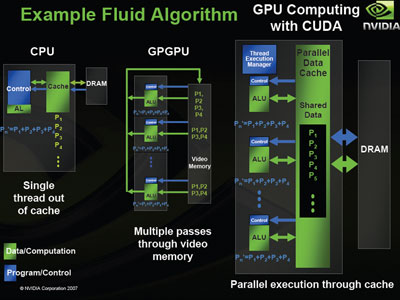
\includegraphics[width=.5\linewidth]{pic/cuda.jpg}
%    \caption{Something about CUDA architecture. Quite interesting.}
%    \label{fig:cuda}
%\end{figure}

%    \begin{table}
%        \centering
%        \begin{tabular}{@{}lrr@{}} 
%            \toprule
%            \multicolumn{2}{c}{Education}\\ \cmidrule{1-2}
%            Major & Duration & Income (\euro)\\ 
%            \midrule 
%            CompSci & 2 & 12,75 \\ \addlinespace
%            MST & 6 & 8,20 \\ \addlinespace
%            VWL & 14 & 10,00\\ 
%            \bottomrule
%        \end{tabular}
%        \caption[Table Example]{A basic example from the booktabs package.}
%        \label{tab::ex}
%    \end{table}

%\begin{abstract} \end{abstract} \section{Introduction} \section{Related Work} \section{Methods} \section{Results} \section{Conclusion}

% USEFUL NOTES END ------------------------------------------------------------

%TODO: QUESTIONS:
% - 

\begin{document}
%
\frontmatter          % for the preliminaries
%
\pagestyle{headings}  % switches on printing of running heads
%
\mainmatter              % start of the contributions
%
\title{Article review: IMAGENET-TRAINED CNNS ARE BIASED TOWARDS TEXTURE; INCREASING SHAPE BIAS IMPROVES ACCURACY AND ROBUSTNESS}
\subtitle{Seminar: Vision Systems MA-INF 4208 \\by prof. Sven Behnke and Hafez Farazi}
%
\titlerunning{Seminar: Vision Systems}  % abbreviated title (for running head)
%
\author{Beaumont, Fabrice}
%
\authorrunning{Beaumont, Fabrice}   % abbreviated author list (for running head)
\institute{Universit\"at Bonn\\
\email{s6fabeau@uni-bonn.de},
Matrikelnummer: 2747609
}

\maketitle              % typeset the title of the contribution

\begin{abstract}
	Convolutional Neural Networks (CNNs) are used for many Computer Vision tasks and yet not all factors of their success are fully understood. In this paper I will summarize the results of the paper ``IMAGENET-TRAINED CNNS ARE BIASED TOWARDS TEXTURE; INCREASING SHAPE BIAS IMPROVES ACCURACY AND ROBUSTNESS'' which was published as a conference paper at ICLR in 2019 \citep{geirhos2018imagenet}. These results indicate that depending on the database used for training, CNNs can bias their recognition towards recognized shape or texture. The authors of this paper also find, that CNNs which are biased towards shape perform better due to a higher tolerance of noise and a better transfer learning. I will conclude the summary with some criticism towards the argumentation and questions left uncommented by the authors. At last I will offer some suggestions for future work, since this is missing in the summarized paper entirely.
\end{abstract}

\section{Introduction}

In this paper I will summarize the paper ``IMAGENET-TRAINED CNNS ARE BIASED TOWARDS TEXTURE; INCREASING SHAPE BIAS IMPROVES ACCURACY AND ROBUSTNESS'' by Robert Geirhos, Patricia Rubisch, Claudio Michaelis, Matthias Bethge, Felix A. Wichmann and Wieland Brendel from 2018 \citep{geirhos2018imagenet}.\\
There are three main results of this paper. 
First, they conclude from a set of experiments that convolutional neural nets (CNNs) use textures for classifications on the ImageNet database. Secondly, they show that this texture-bias can be replaced by a shape-bias by using an adapted database. Finally the authors present experiments, which indicate that CNNs with a shape-bias are more robust to unseen distortions and noise.\\

After the summary of this paper I will offer some criticism on it and give some inspiration for future work.


\subsection{The object detection task}
%(till 1. page)
Object recognition and semantic segmentation are common tasks in Computer Vision 
. CNNs have been regarded as the closest model of the human vision \citep{kubilius2016}, \cite{ritter2017cognitive}, \cite{cadieu2014deep}, \citep{yamins2014performance} and suited for object recognition task and related tasks \citep{krizhevsky2012imagenet}, \cite{long2015fully}.

The fundamental question which the experiments of the authors should answer was, on which visual cues a CNN base their classification. To guide the experiments, they identify two different hypothesis to this question: The experiments should answer if a CNN bases its classification on the shape or texture which is present in the presented image. They refer to these opposing answers as the shape and the texture hypothesis and base them on the literature they are referring to in the paper.\\

The authors stress, that this shape hypothesis is considered as ``one widely accepted intuition''\citep{geirhos2018imagenet}. Furthermore, it justifies the usage of CNNs as a model of the human ventral system \citep{cadieu2014deep}, \citep{yamins2014performance}. On the other hand, the authors refer to a lot more literature, which indicates that the texture hypothesis might be more accurate.\\

Since the authors present a variety of different of related work in context of these two hypothesis, I will give an overview about it in the next section.

\section{Related work}

\subsection{Shape hypothesis}
In this context the shape hypothesis states, that CNNs base their image classification on the shape of an object, found in a presented image. Publications, which indicate that this hypothesis is true and were used by the authors are the following:\\
\citep{zeiler2014visualizing} found, that visualizing the functionality of neural networks in CNNs indicates that their learn to recognize object parts - often interpreted as shapes \citep{ritter2017cognitive}. One such proposed method of visualization are Deconvolutional Networks. \citep{ritter2017cognitive}, \citep{cadieu2014deep}, \cite{yamins2014performance} and \citep{landau1988importance} imply, that CNNs were at the time the most predictive models for the human ventral stream object recognition, which is biased towards object shape.

\subsection{Texture hypothesis}
In this context the texture hypothesis states, that CNsN base their image classification on the texture, found in a presented image.  Publications, which indicate that this hypothesis is true and were used by the authors are the following:

It had been proposed by \citep{ritter2017cognitive} and supported by \citep{geirhos2018generalisation} that CNNs tend to use shape rather than colour in order to categorize objects. But \citep{hosseini2018assessingo} argued, that CNNs perform significantly different on images with reversed brightness (negative images) - which arguable preserve all shapes from the original image. Thus they conclude that shape can not be the only deciding factor.

\citep{gatys2015texture}, \citep{gatys2017controlling}, \citep{brendel2019approximating}, \citep{ballester2016performance}, \citep{funke2017synthesising}, \citep{ballester2016performance} and \citep{eckstein2017beyond} all observed, that CNNs continue to perform well, if the shape of the presented objects was distorted or missing but perform badly, if the texture is missing.

On top of that, \citep{wallis2017parametric}, \citep{laskar2018correspondence} and\citep{long2018role} argued, that the correlation between CNNs and the human ventral stream could be based around their ability to recognize texture and not shape.

With these publications in mind, the Geirhos and his team aimed towards specifying the prominent cues on which classifications done by a CNN are based on. In the next section their methods to achieve this goal are summarized.

\section{Methods}
The authors present three major results. As indicated by their presentation in the paper, these results and the methods used to support them follow a natural order. First, so investigate whether CNNs are biased towards shape or texture, the authors use the classifications of 97 humans as a comparison against the performance of four CNNs. It is reasonable since it is supported by some publications that humans base their object recognition on shape, rather than texture \citep{ritter2017cognitive}, \citep{landau1988importance}.\\

For these experiments, images in the categories original, greyscale, silhouette, object shape, texture  and texture-cue conflict were presented to both the humans and the CNN. Images of the class original, were 160 untempered images from the database ImageNet. They show objects in natural colour in front of a white background.
Images of the class greyscale, silhouette and object shape, were converted images from the original class. For this convertation the authors used skimage.color.rgb2gray, a series of command line convertations with commands like convert and potrace, manual adjustment to pixels of the images and the Canny edge extractor implemented in MATLAB).
For each of these classes 160 images were used. Images of the class texture were original images in natural colour from the database ImageNet, too. But they typically displayed patches of an animal or many repetitions of the same man-made objects. 48 of these pictures were used. Finally, images of the class texture-cue conflict, were generated using the method of style-transfer (implemented by Huang and Belongie \citep{huang2017arbitrary}).

This method was originally proposed by Gatys and his team in 2016 \citep{gatys2016image}. It merges the content of one picture - in this case an image from the class original - with the style of another picture - in this case an image from the class texture. This merge process strips the content picture of its texture and replaces the latter with the texture of the style picture. This way the results contain shapes displaying one object and a texture that belongs to another object. 1280 of these images were used.\\

All images displayed an equal amount of shapes from 16 different categories. They are called the 16-class-ImageNet categories and where introduced by Geirhos et al. in 2018.%TODO
These 16 categories are airplane, bear, bicycle, bird, boat, bottle, car, cat, chair, clock, dog, elephant, keyboard, knife, oven and truck. Note that the images of the texture-cue conflict class only the underlying shape image has to correspond to one of these categories.


%(till 2. page)
\subsection{Experimental setup}
The experimental setup for the four CNNs contains of a direct application of the pre-trained algorithms to the described categories. Both all the images from the class original and texture were correctly classified by all four pre-trained CNNs. \\

For the trials involving humans each trial lasted 2200 ms and contained the display of a fixation square (300 ms), a stimulus image (200 ms), a full-contrast pink noise mask (200 ms) and a screen where the participants had to select one of the 16-class ImageNet categories as their response to the image (1500 ms). One participant was shown pictures of exactly one class only. The participants classifying images with an objective ground true (not the texture-cue conflict images) were motivated by an increase in payment proportional to an accuracy above 50\%. The authors claim, that by following the paradigm of Geirhos et al. from 2018 they would have achieved maximal comparability between the human participants and the CNNs.

\subsection{Result 1 - Supporting the texture hypothesis}
The results indicate, that both the pre-trained CNNs and the human participants perform well in the classification if both the object shape and texture are present (classes original, greyscale and texture). If the texture is missing entirely (classes silhouette and edges) all performances are lower, but the human participants still had an accuracy above 75\% where as the algorithms had one below 54\%.%TODO: Figure 2
When both a shape and a texture cue was present, the human participants showed a clear preference for the identification of the object whose shape was present. On the other hand, the decisions of the algorithms varied much more but was overall more often guided by the present texture.\\ %TODO: Figure 4\\

The authors concluded, that CNNs in general are biased towards texture, whereas humans are biased towards shape. They argued, that this bias is not present by design, but rather  induced by the database used for training. Since one application for the CNNs is to model the human vision, the authors tried to shift the texture bias towards a shape bias, like it can be observed for humans.

%(till 4. page)
\subsection{SIN}
In order to shift the bias of the CNNs, the authors changed the database used for the training. The underlying strategy was to remove the information stored in the texture of the images and only keeping the information stored in the shape of the images in tact. This way the texture information looses importance and the CNNs would have to rely on the shapes.\\
The authors used the same method like for the images in the texture-shape cue conflict class, but this time the source for the style images were the 79.434 paintings images in Kaggle's ``Painter by Number'' data set (\url{https://www.kaggle.com/c/painter-by-numbers/}, which the authors accessed on March 1, 2018).\\

\subsection{Result 2 - Switching to a shape-bias}

The reported experiments indicate, that the classification performed by the ResNet-50 which was trained on SIN has shifted towards the shape recognition when it comes to the texture-shape cue conflict class. They also hint at similar results for the Alexnet and VGG-16.\\

%TODO: Figure 3


Finally the authors tried to determine, if the training with the changed database improves the performance of the CNNs.

\subsection{Result 3 - Superiority of the shape-bias}
Define: BagNets\\
Experiments/results displayed in Figure 4, 5, table 2

Adversarial input.\\

In the paper the authors argue, that a lower top-5 accuracy of the ResNet-50 trained and evaluated on the SIN database (79,0\%) than on the IN database (92.0\%) indicates, that the classification using only shape cues is more difficult. %TODO: They did not consider that the database was simply scewed and contained some non-sense images. Thus it contained noise images and fewer relyable examples
Furthermore, since the evaluation on the other database lead to a significant performance drop if the CNN was trained on the IN database (16.4\%) but an increase if it was trained on the SIN database (82.6\%), the authors argue, that relying on shape is more effective and generalizes better than relying on texture.\\

On top of that, results are presented that indicate that the performance of the ResNet-50 can be increased with respect to the training on the IN database if the SIN databases is used for training additionally. This performance increase is most obvious when the CNN was evaluated on the databases PASCAL VOC and MS COCO. For the evaluation of these two databases the authors used a Fast R-CNN implementation.\\%TODO numbers and image

Finally the authors present results which indicate, that the ResNet-50 trained on the SIN database is much more robust to unseen noise than if trained on the IN database. The tested noise was uniform noise, low contrast-, high- and and low-pass filters and three Eidolon perturbations. %TODO numbers and image

%(till 5. page)
\section{Conclusion}
The summarized paper by Geirhos et al. from 2019 presents experimental results which indicate that CNNs tend to use texture over shape for classification tasks, if the training database allows for this method. Using a modified database can increase the tendency of a CNN to classify images using the displayed shapes. If this is the case, the performance is increased, transfers better to unseen data including noise.\\

The authors demonstrate these findings for one kind of database adaptation using the ImageNet database, a style-transfer method and Kaggle's ``Painter by Number'' data set.%TODO: 
The results focus on experiments with implementations of ResNet-50.

%(till 6. page)
\section{Critic}
The overall structure of the paper is very clear and simple to follow. The train of thought leads the reader in a logical comprehensive way from one result to the next. All presented images, figures and tables support the understanding and underline the presented information.
On top of that, the appendix hints at more detailed findings and completes the main paper seamlessly.\\

Nevertheless there are some weak points of the paper. Most obvious is the missing section about future work and an outlook on how to use and further investigate the presented results.
Secondly, some assumptions regarding the first major result can be challenged. For example the authors interpret the lower top5-accuracy of the ResNet50 trained and evaluated on the SIN database as an indication that classification by shape is more difficult for the algorithm. In this argumentation they seem to not consider, that based on their construction of the SIN database, some images may loose information about the displayed object shape during the style-transfer. Thus the algorithm has less reliable input to train and evaluate on. This leads to the following other weak point of the paper. The authors themselves do acknowledge that the style-transfer can lead to images without reliable information about the object shape, but they do not implement or suggest any methods to counter this problem. Since the underlying idea of the SIN database is to have reliable shape information, counter measures seem to be essential. One example would be to use high-pass filters or otherwise increase the clarity of edges and shapes. This could be done both before the style-transfer and later added to the image or afterwards. The methods to derive the object silhouette or the edge shapes could be applied too.\\
Next, the authors only experiment with one kind of style-transfer by relying on one database of pictures for the artificial textures only. It seems to be a natural question to ask how other kinds of style-transfer are able to change biases in CNNs.\\
Related to this question is, how other parameters such as changes to the architecture of the CNN or usage of loss functions can influence any present bias.\\

On a less general base, the authors do not comment what happened during the so called ``fine tuning''-step for the Shape-ResNet. It has a rather noticable positive effect on its performance. For the results with respect to the MS COCO this improvement is just slightly less, than the actual additional usage of the SIN itself.\\
On top of that, the reasons for the decision to focus on ResNet-50 are not very clear. While similar results with other CNNs are hinted at, the authors formulate the last two results as general statements, but only support the claims with results about this single CNN.\\

Lastly, the authors state that all the images from the class original and texture were correctly classified by all four pre-trained CNNs. Thus it is misleading, that the perfect accuracy of the CNNs regarding the recognition task for not only the greyscale, silhouette, object shape and texture-cure conflict images, but also the original and texture images are presented. By construction the latter are recognized perfectly and thus this result gives no indication about the actual performance of the CNNs.

%Why was only ONE cure conflict shape-texture used?Why not alternative parameters like colour, amount of objects,\dots?\\
%
%Idea of SIN was to make the texture a noisance, keep the shape intactBut, as stated by the authors: ``a substantial fraction'' (2019, Geirhos et al., page 5) of output from the style-transfer was not recognizable (non-sense images). Why were no counter measures used? E.g. preserving the edges.\\
%
%Can the initially expected shape-hierarchy be interpreted as a texture-hierarchy?How does the Shape-ResNet looks in the inside? (Deconvolutional NN, Feature visualization)What is the possible ``error'' in the shape-hierarchy-hypothesis? \\
%
%Does the Shape-ResNet perform better on negative images? (This was the mentioned counter example against the shape-hypothesis given by Hosseini et al. in 2018)\\
%
%The improvements by the usage of SIN were much more prominent with the experiments with the Faster-RCNN implementation (by Ren et la., 2017) (Pascal VOC, MS COCO databases). Is this only database related or maybe related to the implementation, too?\\
%
%How was the performance agains adverserial input? What kind of adverserial input can fool the Shape-ResNet?
%``\dots still susceptible to adversarial examples\dots'' Geirhos to ``The Register'' 2020; https://www.theregister.com/2019/02/13/ai_image_texture/\\
%
%Why was there no comment on Between-Class learning (Mix-up technique)? (e.g. Tokozume et al., 2018 and after the publication:  Bhattacharjee et al. 2020)Is it possible that different biases lead to categorically different object detections?\\

A „future work“ section is missing\\

\section{Future work}

From this paper one can derive many questions for future investigations with respect to the learning performed by CNNs. Arguably the authors only experimented with one kind of stylization by using one style-transfer method \citep{huang2017arbitrary} and one specific data base for the style images which consisted of paintings (Kaggle's ``Painter by Numbers''). \citep{hosseini2018assessing} experimented with the performance of CNNs on images that where modified in a different way. They used inverted images which loose some information about the original color but preserve all information about edges and thus shape. One could expand these experiments in order to investigate what kind of databases are most suited for what kind of recognition tasks. Also, it would be interesting to what extent the underlying decision process of CNNs can be determined by augmenting the training database.

In contrast to this, it remains unclear, if similar biases of CNNs can be induced by changing their architecture or introducing loss functions to the network. Afterwards one could try to combine several of these approaches to further guide the decision parameters of CNNs.

On the other hand, it could be disadvantageous to have CNNs that are strongly biased towards single cues like only object shape. Depending on the complexity of the target database it could be promising to add a decision layer for the CNNs, which applies classification mechanisms with different biases, depending on the already found information. The texture of some object are arguably more important than its shape. One very basic natural occurring example is the distinction between different panthers such as the black panther, a leopard or a jaguar.

At last, the authors of the presented paper use the object classification task for their evaluation. The application and evaluation of their method to other related tasks in the field of Computer Vision could be investigated too. For example the task of semantic segmentation could be further specified, if different biases of the used CNNs lead to different but arguable useful segmentations.

\printbibliography
\end{document}
